\documentclass[1p]{elsarticle_modified}
%\bibliographystyle{elsarticle-num}

%\usepackage[colorlinks]{hyperref}
%\usepackage{abbrmath_seonhwa} %\Abb, \Ascr, \Acal ,\Abf, \Afrak
\usepackage{amsfonts}
\usepackage{amssymb}
\usepackage{amsmath}
\usepackage{amsthm}
\usepackage{scalefnt}
\usepackage{amsbsy}
\usepackage{kotex}
\usepackage{caption}
\usepackage{subfig}
\usepackage{color}
\usepackage{graphicx}
\usepackage{xcolor} %% white, black, red, green, blue, cyan, magenta, yellow
\usepackage{float}
\usepackage{setspace}
\usepackage{hyperref}

\usepackage{tikz}
\usetikzlibrary{arrows}

\usepackage{multirow}
\usepackage{array} % fixed length table
\usepackage{hhline}

%%%%%%%%%%%%%%%%%%%%%
\makeatletter
\renewcommand*\env@matrix[1][\arraystretch]{%
	\edef\arraystretch{#1}%
	\hskip -\arraycolsep
	\let\@ifnextchar\new@ifnextchar
	\array{*\c@MaxMatrixCols c}}
\makeatother %https://tex.stackexchange.com/questions/14071/how-can-i-increase-the-line-spacing-in-a-matrix
%%%%%%%%%%%%%%%

\usepackage[normalem]{ulem}

\newcommand{\msout}[1]{\ifmmode\text{\sout{\ensuremath{#1}}}\else\sout{#1}\fi}
%SOURCE: \msout is \stkout macro in https://tex.stackexchange.com/questions/20609/strikeout-in-math-mode

\newcommand{\cancel}[1]{
	\ifmmode
	{\color{red}\msout{#1}}
	\else
	{\color{red}\sout{#1}}
	\fi
}

\newcommand{\add}[1]{
	{\color{blue}\uwave{#1}}
}

\newcommand{\replace}[2]{
	\ifmmode
	{\color{red}\msout{#1}}{\color{blue}\uwave{#2}}
	\else
	{\color{red}\sout{#1}}{\color{blue}\uwave{#2}}
	\fi
}

\newcommand{\Sol}{\mathcal{S}} %segment
\newcommand{\D}{D} %diagram
\newcommand{\A}{\mathcal{A}} %arc


%%%%%%%%%%%%%%%%%%%%%%%%%%%%%5 test

\def\sl{\operatorname{\textup{SL}}(2,\Cbb)}
\def\psl{\operatorname{\textup{PSL}}(2,\Cbb)}
\def\quan{\mkern 1mu \triangleright \mkern 1mu}

\theoremstyle{definition}
\newtheorem{thm}{Theorem}[section]
\newtheorem{prop}[thm]{Proposition}
\newtheorem{lem}[thm]{Lemma}
\newtheorem{ques}[thm]{Question}
\newtheorem{cor}[thm]{Corollary}
\newtheorem{defn}[thm]{Definition}
\newtheorem{exam}[thm]{Example}
\newtheorem{rmk}[thm]{Remark}
\newtheorem{alg}[thm]{Algorithm}

\newcommand{\I}{\sqrt{-1}}
\begin{document}

%\begin{frontmatter}
%
%\title{Boundary parabolic representations of knots up to 8 crossings}
%
%%% Group authors per affiliation:
%\author{Yunhi Cho} 
%\address{Department of Mathematics, University of Seoul, Seoul, Korea}
%\ead{yhcho@uos.ac.kr}
%
%
%\author{Seonhwa Kim} %\fnref{s_kim}}
%\address{Center for Geometry and Physics, Institute for Basic Science, Pohang, 37673, Korea}
%\ead{ryeona17@ibs.re.kr}
%
%\author{Hyuk Kim}
%\address{Department of Mathematical Sciences, Seoul National University, Seoul 08826, Korea}
%\ead{hyukkim@snu.ac.kr}
%
%\author{Seokbeom Yoon}
%\address{Department of Mathematical Sciences, Seoul National University, Seoul, 08826,  Korea}
%\ead{sbyoon15@snu.ac.kr}
%
%\begin{abstract}
%We find all boundary parabolic representation of knots up to 8 crossings.
%
%\end{abstract}
%\begin{keyword}
%    \MSC[2010] 57M25 
%\end{keyword}
%
%\end{frontmatter}

%\linenumbers
%\tableofcontents
%
\newcommand\colored[1]{\textcolor{white}{\rule[-0.35ex]{0.8em}{1.4ex}}\kern-0.8em\color{red} #1}%
%\newcommand\colored[1]{\textcolor{white}{ #1}\kern-2.17ex	\textcolor{white}{ #1}\kern-1.81ex	\textcolor{white}{ #1}\kern-2.15ex\color{red}#1	}

{\Large $\underline{12n_{0427}~(K12n_{0427})}$}

\setlength{\tabcolsep}{10pt}
\renewcommand{\arraystretch}{1.6}
\vspace{1cm}\begin{tabular}{m{100pt}>{\centering\arraybackslash}m{274pt}}
\multirow{5}{120pt}{
	\centering
	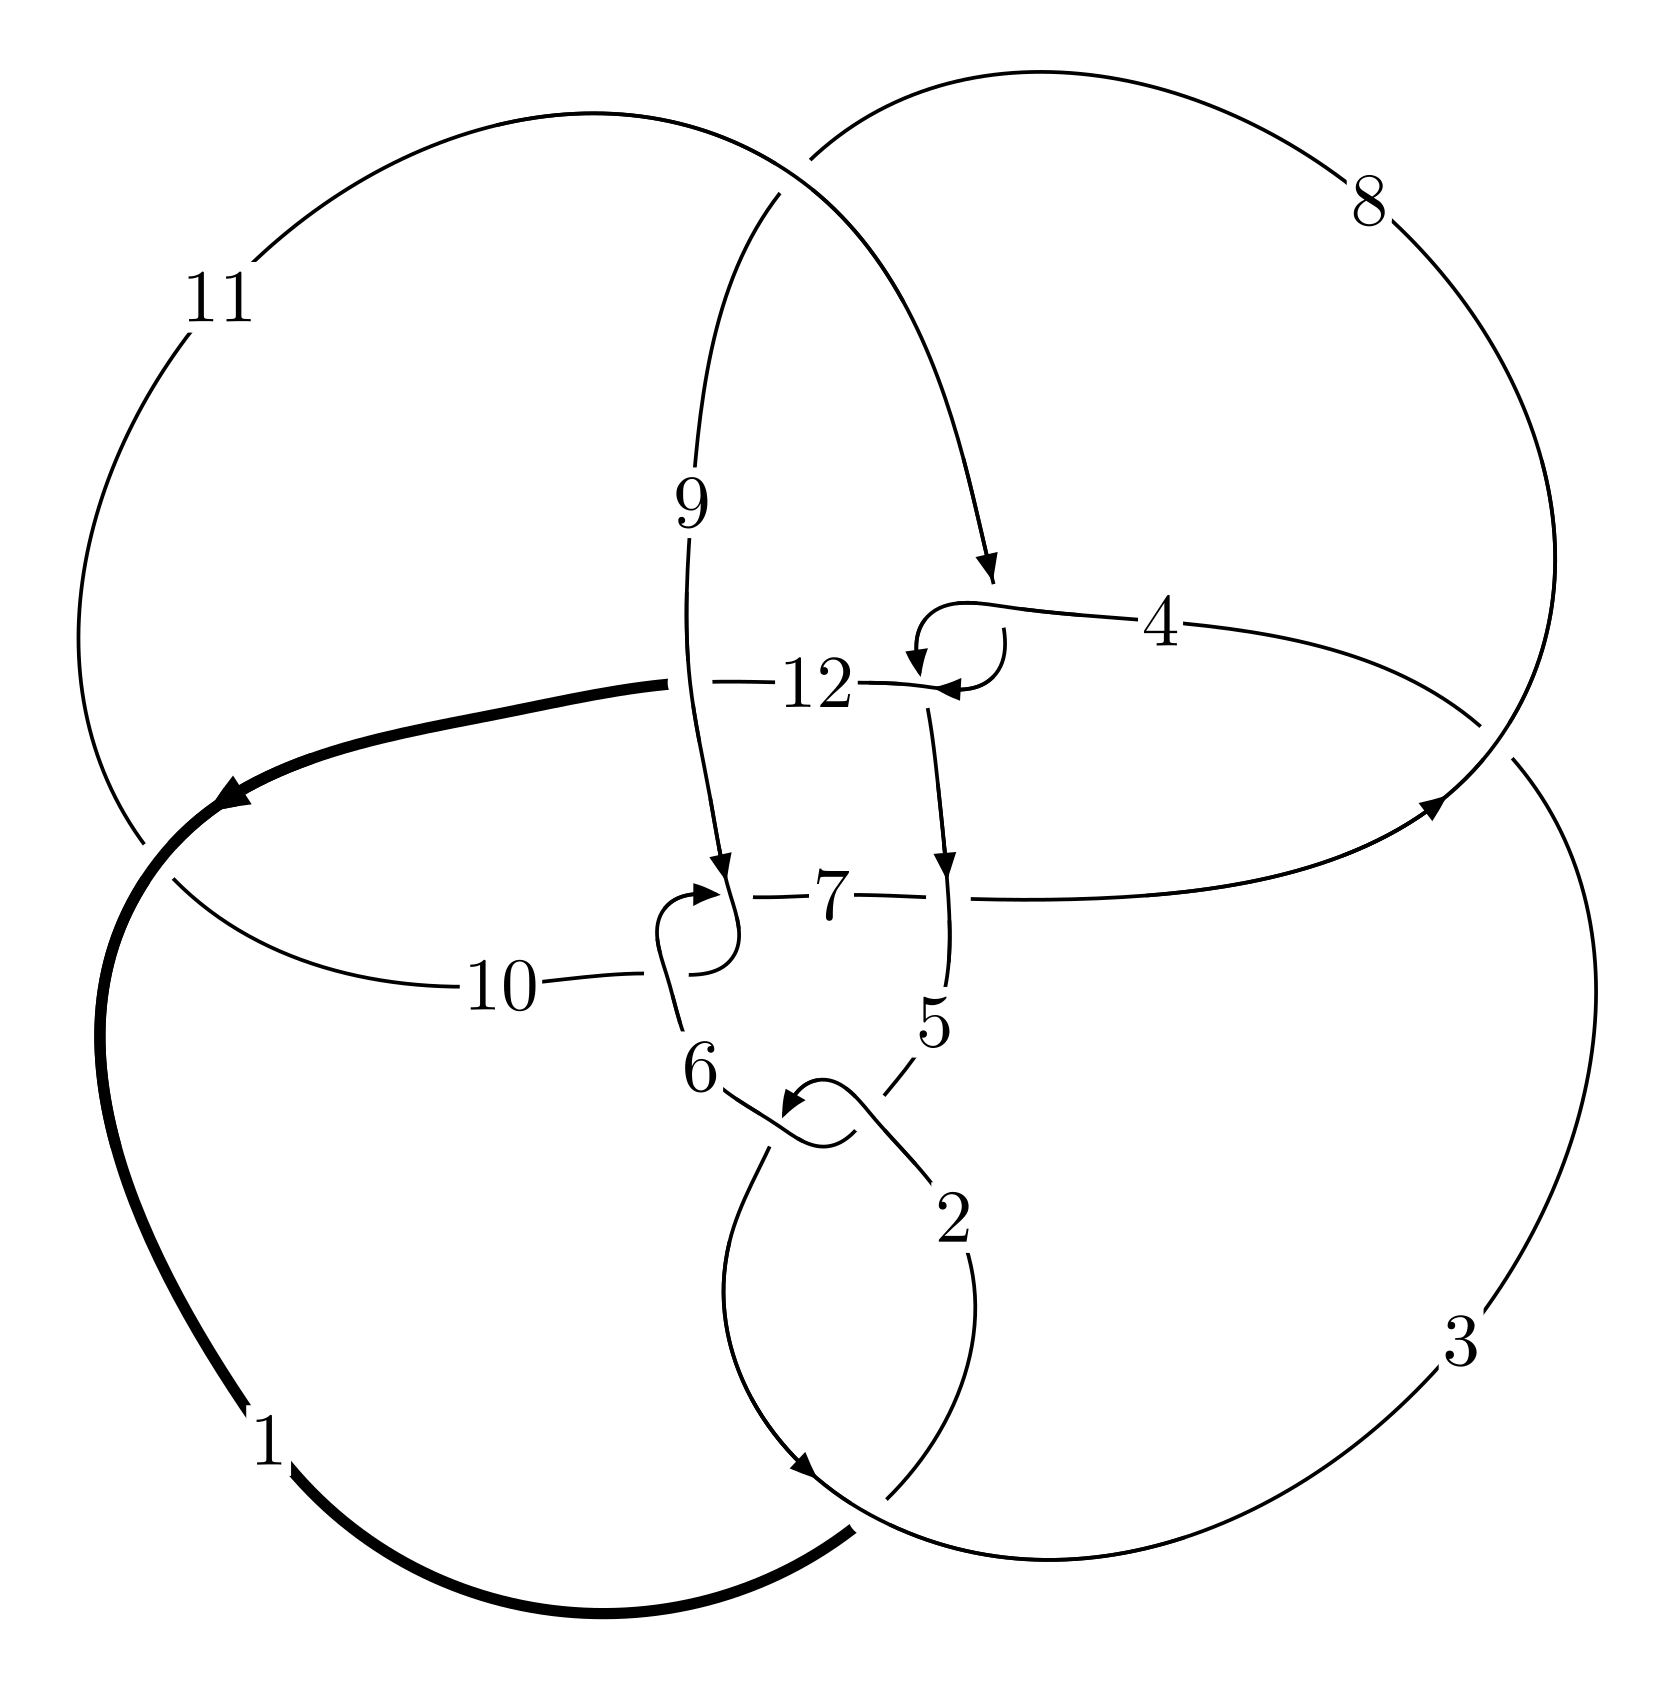
\includegraphics[width=112pt]{../../../GIT/diagram.site/Diagrams/png/2516_12n_0427.png}\\
\ \ \ A knot diagram\footnotemark}&
\allowdisplaybreaks
\textbf{Linearized knot diagam} \\
\cline{2-2}
 &
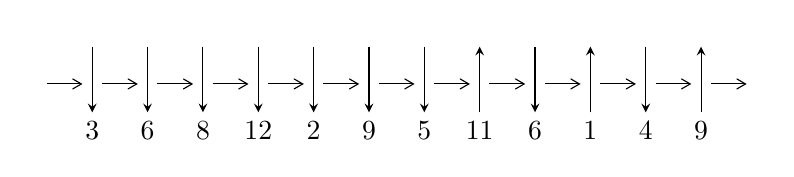
\begin{tikzpicture}[x=20pt, y=17pt]
	% nodes
	\node (C0) at (0, 0) {};
	\node (C1) at (1, 0) {};
	\node (C1U) at (1, +1) {};
	\node (C1D) at (1, -1) {3};

	\node (C2) at (2, 0) {};
	\node (C2U) at (2, +1) {};
	\node (C2D) at (2, -1) {6};

	\node (C3) at (3, 0) {};
	\node (C3U) at (3, +1) {};
	\node (C3D) at (3, -1) {8};

	\node (C4) at (4, 0) {};
	\node (C4U) at (4, +1) {};
	\node (C4D) at (4, -1) {12};

	\node (C5) at (5, 0) {};
	\node (C5U) at (5, +1) {};
	\node (C5D) at (5, -1) {2};

	\node (C6) at (6, 0) {};
	\node (C6U) at (6, +1) {};
	\node (C6D) at (6, -1) {9};

	\node (C7) at (7, 0) {};
	\node (C7U) at (7, +1) {};
	\node (C7D) at (7, -1) {5};

	\node (C8) at (8, 0) {};
	\node (C8U) at (8, +1) {};
	\node (C8D) at (8, -1) {11};

	\node (C9) at (9, 0) {};
	\node (C9U) at (9, +1) {};
	\node (C9D) at (9, -1) {6};

	\node (C10) at (10, 0) {};
	\node (C10U) at (10, +1) {};
	\node (C10D) at (10, -1) {1};

	\node (C11) at (11, 0) {};
	\node (C11U) at (11, +1) {};
	\node (C11D) at (11, -1) {4};

	\node (C12) at (12, 0) {};
	\node (C12U) at (12, +1) {};
	\node (C12D) at (12, -1) {9};
	\node (C13) at (13, 0) {};

	% arrows
	\draw[->,>={angle 60}]
	(C0) edge (C1) (C1) edge (C2) (C2) edge (C3) (C3) edge (C4) (C4) edge (C5) (C5) edge (C6) (C6) edge (C7) (C7) edge (C8) (C8) edge (C9) (C9) edge (C10) (C10) edge (C11) (C11) edge (C12) (C12) edge (C13) ;	\draw[->,>=stealth]
	(C1U) edge (C1D) (C2U) edge (C2D) (C3U) edge (C3D) (C4U) edge (C4D) (C5U) edge (C5D) (C6U) edge (C6D) (C7U) edge (C7D) (C8D) edge (C8U) (C9U) edge (C9D) (C10D) edge (C10U) (C11U) edge (C11D) (C12D) edge (C12U) ;
	\end{tikzpicture} \\
\hhline{~~} \\& 
\textbf{Solving Sequence} \\ \cline{2-2} 
 &
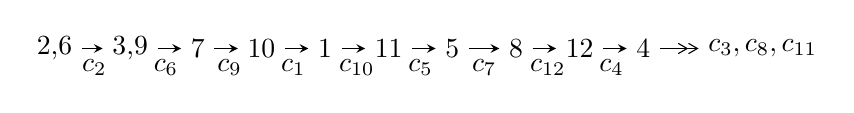
\begin{tikzpicture}[x=23pt, y=7pt]
	% node
	\node (A0) at (-1/8, 0) {2,6};
	\node (A1) at (17/16, 0) {3,9};
	\node (A2) at (17/8, 0) {7};
	\node (A3) at (25/8, 0) {10};
	\node (A4) at (33/8, 0) {1};
	\node (A5) at (41/8, 0) {11};
	\node (A6) at (49/8, 0) {5};
	\node (A7) at (57/8, 0) {8};
	\node (A8) at (65/8, 0) {12};
	\node (A9) at (73/8, 0) {4};
	\node (C1) at (1/2, -1) {$c_{2}$};
	\node (C2) at (13/8, -1) {$c_{6}$};
	\node (C3) at (21/8, -1) {$c_{9}$};
	\node (C4) at (29/8, -1) {$c_{1}$};
	\node (C5) at (37/8, -1) {$c_{10}$};
	\node (C6) at (45/8, -1) {$c_{5}$};
	\node (C7) at (53/8, -1) {$c_{7}$};
	\node (C8) at (61/8, -1) {$c_{12}$};
	\node (C9) at (69/8, -1) {$c_{4}$};
	\node (A10) at (11, 0) {$c_{3},c_{8},c_{11}$};

	% edge
	\draw[->,>=stealth]	
	(A0) edge (A1) (A1) edge (A2) (A2) edge (A3) (A3) edge (A4) (A4) edge (A5) (A5) edge (A6) (A6) edge (A7) (A7) edge (A8) (A8) edge (A9) ;
	\draw[->>,>={angle 60}]	
	(A9) edge (A10);
\end{tikzpicture} \\ 

\end{tabular} \\

\footnotetext{
The image of knot diagram is generated by the software ``\textbf{Draw programme}" developed by Andrew Bartholomew(\url{http://www.layer8.co.uk/maths/draw/index.htm\#Running-draw}), where we modified some parts for our purpose(\url{https://github.com/CATsTAILs/LinksPainter}).
}\phantom \\ \newline 
\centering \textbf{Ideals for irreducible components\footnotemark of $X_{\text{par}}$} 
 
\begin{align*}
I^u_{1}&=\langle 
-9.07936\times10^{110} u^{78}+8.79010\times10^{109} u^{77}+\cdots+6.15846\times10^{109} b-9.76189\times10^{110},\\
\phantom{I^u_{1}}&\phantom{= \langle  }5.98068\times10^{109} u^{78}-1.62667\times10^{110} u^{77}+\cdots+6.15846\times10^{109} a+1.72158\times10^{110},\;u^{79}- u^{78}+\cdots-5 u-1\rangle \\
I^u_{2}&=\langle 
-12 u^{22}+36 u^{21}+\cdots+29 b+62,\;17 u^{22}+65 u^{21}+\cdots+29 a+178,\;u^{23}-6 u^{21}+\cdots+3 u-1\rangle \\
\\
\end{align*}
\raggedright * 2 irreducible components of $\dim_{\mathbb{C}}=0$, with total 102 representations.\\
\footnotetext{All coefficients of polynomials are rational numbers. But the coefficients are sometimes approximated in decimal forms when there is not enough margin.}
\newpage
\renewcommand{\arraystretch}{1}
\centering \section*{I. $I^u_{1}= \langle -9.08\times10^{110} u^{78}+8.79\times10^{109} u^{77}+\cdots+6.16\times10^{109} b-9.76\times10^{110},\;5.98\times10^{109} u^{78}-1.63\times10^{110} u^{77}+\cdots+6.16\times10^{109} a+1.72\times10^{110},\;u^{79}- u^{78}+\cdots-5 u-1 \rangle$}
\flushleft \textbf{(i) Arc colorings}\\
\begin{tabular}{m{7pt} m{180pt} m{7pt} m{180pt} }
\flushright $a_{2}=$&$\begin{pmatrix}1\\0\end{pmatrix}$ \\
\flushright $a_{6}=$&$\begin{pmatrix}0\\u\end{pmatrix}$ \\
\flushright $a_{3}=$&$\begin{pmatrix}1\\u^2\end{pmatrix}$ \\
\flushright $a_{9}=$&$\begin{pmatrix}-0.971132 u^{78}+2.64136 u^{77}+\cdots+6.04319 u-2.79547\\14.7429 u^{78}-1.42732 u^{77}+\cdots+94.4842 u+15.8512\end{pmatrix}$ \\
\flushright $a_{7}=$&$\begin{pmatrix}11.8768 u^{78}-3.37720 u^{77}+\cdots+83.6913 u+11.1756\\11.9659 u^{78}-4.59087 u^{77}+\cdots+116.379 u+18.6517\end{pmatrix}$ \\
\flushright $a_{10}=$&$\begin{pmatrix}-0.971132 u^{78}+2.64136 u^{77}+\cdots+6.04319 u-2.79547\\16.3558 u^{78}-0.971234 u^{77}+\cdots+101.864 u+17.5214\end{pmatrix}$ \\
\flushright $a_{1}=$&$\begin{pmatrix}- u^2+1\\- u^4\end{pmatrix}$ \\
\flushright $a_{11}=$&$\begin{pmatrix}-0.810554 u^{78}+3.36782 u^{77}+\cdots-7.29319 u-4.32558\\12.4497 u^{78}-0.403268 u^{77}+\cdots+72.5802 u+12.6725\end{pmatrix}$ \\
\flushright $a_{5}=$&$\begin{pmatrix}u\\u\end{pmatrix}$ \\
\flushright $a_{8}=$&$\begin{pmatrix}12.8514 u^{78}-3.04231 u^{77}+\cdots+89.2245 u+12.3001\\12.9406 u^{78}-4.25598 u^{77}+\cdots+121.912 u+19.7762\end{pmatrix}$ \\
\flushright $a_{12}=$&$\begin{pmatrix}-14.4160 u^{78}+5.24384 u^{77}+\cdots-95.6278 u-14.3701\\-11.5538 u^{78}+3.34984 u^{77}+\cdots-112.598 u-17.7373\end{pmatrix}$ \\
\flushright $a_{4}=$&$\begin{pmatrix}17.1980 u^{78}-7.17604 u^{77}+\cdots+116.184 u+19.2207\\6.15055 u^{78}-3.28266 u^{77}+\cdots+78.6335 u+11.8437\end{pmatrix}$\\&\end{tabular}
\flushleft \textbf{(ii) Obstruction class $= -1$}\\~\\
\flushleft \textbf{(iii) Cusp Shapes $= 13.0730 u^{78}-4.80433 u^{77}+\cdots+106.377 u+11.6389$}\\~\\
\newpage\renewcommand{\arraystretch}{1}
\flushleft \textbf{(iv) u-Polynomials at the component}\newline \\
\begin{tabular}{m{50pt}|m{274pt}}
Crossings & \hspace{64pt}u-Polynomials at each crossing \\
\hline $$\begin{aligned}c_{1}\end{aligned}$$&$\begin{aligned}
&u^{79}+47 u^{78}+\cdots-15 u+1
\end{aligned}$\\
\hline $$\begin{aligned}c_{2},c_{5}\end{aligned}$$&$\begin{aligned}
&u^{79}+u^{78}+\cdots-5 u+1
\end{aligned}$\\
\hline $$\begin{aligned}c_{3}\end{aligned}$$&$\begin{aligned}
&u^{79}+2 u^{78}+\cdots-1585 u-751
\end{aligned}$\\
\hline $$\begin{aligned}c_{4},c_{11}\end{aligned}$$&$\begin{aligned}
&u^{79}+u^{78}+\cdots-95 u-17
\end{aligned}$\\
\hline $$\begin{aligned}c_{6},c_{9}\end{aligned}$$&$\begin{aligned}
&u^{79}+8 u^{78}+\cdots+228781 u+27293
\end{aligned}$\\
\hline $$\begin{aligned}c_{7}\end{aligned}$$&$\begin{aligned}
&u^{79}-10 u^{78}+\cdots+105789720 u-12203621
\end{aligned}$\\
\hline $$\begin{aligned}c_{8}\end{aligned}$$&$\begin{aligned}
&u^{79}+9 u^{78}+\cdots+87 u+1
\end{aligned}$\\
\hline $$\begin{aligned}c_{10}\end{aligned}$$&$\begin{aligned}
&u^{79}+6 u^{78}+\cdots+180673434 u+11333737
\end{aligned}$\\
\hline $$\begin{aligned}c_{12}\end{aligned}$$&$\begin{aligned}
&u^{79}-3 u^{78}+\cdots-427561 u+16969
\end{aligned}$\\
\hline
\end{tabular}\\~\\
\newpage\renewcommand{\arraystretch}{1}
\flushleft \textbf{(v) Riley Polynomials at the component}\newline \\
\begin{tabular}{m{50pt}|m{274pt}}
Crossings & \hspace{64pt}Riley Polynomials at each crossing \\
\hline $$\begin{aligned}c_{1}\end{aligned}$$&$\begin{aligned}
&y^{79}-23 y^{78}+\cdots+201 y-1
\end{aligned}$\\
\hline $$\begin{aligned}c_{2},c_{5}\end{aligned}$$&$\begin{aligned}
&y^{79}-47 y^{78}+\cdots-15 y-1
\end{aligned}$\\
\hline $$\begin{aligned}c_{3}\end{aligned}$$&$\begin{aligned}
&y^{79}-18 y^{78}+\cdots+14546249 y-564001
\end{aligned}$\\
\hline $$\begin{aligned}c_{4},c_{11}\end{aligned}$$&$\begin{aligned}
&y^{79}-59 y^{78}+\cdots-10729 y-289
\end{aligned}$\\
\hline $$\begin{aligned}c_{6},c_{9}\end{aligned}$$&$\begin{aligned}
&y^{79}-86 y^{78}+\cdots+37605309847 y-744907849
\end{aligned}$\\
\hline $$\begin{aligned}c_{7}\end{aligned}$$&$\begin{aligned}
&y^{79}-74 y^{78}+\cdots+3831097413487084 y-148928365511641
\end{aligned}$\\
\hline $$\begin{aligned}c_{8}\end{aligned}$$&$\begin{aligned}
&y^{79}+17 y^{78}+\cdots+4035 y-1
\end{aligned}$\\
\hline $$\begin{aligned}c_{10}\end{aligned}$$&$\begin{aligned}
&y^{79}+72 y^{78}+\cdots+6604146335611458 y-128453594385169
\end{aligned}$\\
\hline $$\begin{aligned}c_{12}\end{aligned}$$&$\begin{aligned}
&y^{79}+57 y^{78}+\cdots+62831435943 y-287946961
\end{aligned}$\\
\hline
\end{tabular}\\~\\
\newpage\flushleft \textbf{(vi) Complex Volumes and Cusp Shapes}
$$\begin{array}{c|c|c}  
\text{Solutions to }I^u_{1}& \I (\text{vol} + \sqrt{-1}CS) & \text{Cusp shape}\\
 \hline 
\begin{aligned}
u &= -0.124050 + 0.993308 I \\
a &= \phantom{-}0.04579 - 1.50731 I \\
b &= -0.099183 + 0.105938 I\end{aligned}
 & -3.53096 - 5.44418 I & \phantom{-0.000000 } 0 \\ \hline\begin{aligned}
u &= -0.124050 - 0.993308 I \\
a &= \phantom{-}0.04579 + 1.50731 I \\
b &= -0.099183 - 0.105938 I\end{aligned}
 & -3.53096 + 5.44418 I & \phantom{-0.000000 } 0 \\ \hline\begin{aligned}
u &= -1.00792\phantom{ +0.000000I} \\
a &= \phantom{-}1.83576\phantom{ +0.000000I} \\
b &= \phantom{-}3.13845\phantom{ +0.000000I}\end{aligned}
 & -6.57376\phantom{ +0.000000I} & \phantom{-0.000000 } 0 \\ \hline\begin{aligned}
u &= \phantom{-}0.124459 + 1.005840 I \\
a &= -0.20988 - 1.77449 I \\
b &= \phantom{-}0.0137860 - 0.0597242 I\end{aligned}
 & -8.55740 + 11.15110 I & \phantom{-0.000000 } 0 \\ \hline\begin{aligned}
u &= \phantom{-}0.124459 - 1.005840 I \\
a &= -0.20988 + 1.77449 I \\
b &= \phantom{-}0.0137860 + 0.0597242 I\end{aligned}
 & -8.55740 - 11.15110 I & \phantom{-0.000000 } 0 \\ \hline\begin{aligned}
u &= \phantom{-}0.144077 + 0.963515 I \\
a &= \phantom{-}0.42273 - 1.45073 I \\
b &= \phantom{-}0.385199 + 0.154386 I\end{aligned}
 & -7.42668 - 1.34593 I & \phantom{-0.000000 } 0 \\ \hline\begin{aligned}
u &= \phantom{-}0.144077 - 0.963515 I \\
a &= \phantom{-}0.42273 + 1.45073 I \\
b &= \phantom{-}0.385199 - 0.154386 I\end{aligned}
 & -7.42668 + 1.34593 I & \phantom{-0.000000 } 0 \\ \hline\begin{aligned}
u &= \phantom{-}0.860189 + 0.441139 I \\
a &= \phantom{-}1.057870 + 0.073073 I \\
b &= \phantom{-}0.93330 + 1.20699 I\end{aligned}
 & -3.06653 + 2.05333 I & \phantom{-0.000000 } 0 \\ \hline\begin{aligned}
u &= \phantom{-}0.860189 - 0.441139 I \\
a &= \phantom{-}1.057870 - 0.073073 I \\
b &= \phantom{-}0.93330 - 1.20699 I\end{aligned}
 & -3.06653 - 2.05333 I & \phantom{-0.000000 } 0 \\ \hline\begin{aligned}
u &= -0.996413 + 0.319112 I \\
a &= \phantom{-}0.650609 - 1.213410 I \\
b &= \phantom{-}0.649781 - 0.828840 I\end{aligned}
 & -0.44095 + 4.14481 I & \phantom{-0.000000 } 0\\
 \hline 
 \end{array}$$\newpage$$\begin{array}{c|c|c}  
\text{Solutions to }I^u_{1}& \I (\text{vol} + \sqrt{-1}CS) & \text{Cusp shape}\\
 \hline 
\begin{aligned}
u &= -0.996413 - 0.319112 I \\
a &= \phantom{-}0.650609 + 1.213410 I \\
b &= \phantom{-}0.649781 + 0.828840 I\end{aligned}
 & -0.44095 - 4.14481 I & \phantom{-0.000000 } 0 \\ \hline\begin{aligned}
u &= \phantom{-}0.655543 + 0.819980 I \\
a &= \phantom{-}0.255857 + 0.086779 I \\
b &= \phantom{-}0.588626 - 0.201877 I\end{aligned}
 & -0.66585 + 2.44129 I & \phantom{-0.000000 } 0 \\ \hline\begin{aligned}
u &= \phantom{-}0.655543 - 0.819980 I \\
a &= \phantom{-}0.255857 - 0.086779 I \\
b &= \phantom{-}0.588626 + 0.201877 I\end{aligned}
 & -0.66585 - 2.44129 I & \phantom{-0.000000 } 0 \\ \hline\begin{aligned}
u &= \phantom{-}0.967265 + 0.427782 I \\
a &= -0.488566 - 0.371683 I \\
b &= \phantom{-}0.273554 + 0.305272 I\end{aligned}
 & -3.57853 - 3.77822 I & \phantom{-0.000000 } 0 \\ \hline\begin{aligned}
u &= \phantom{-}0.967265 - 0.427782 I \\
a &= -0.488566 + 0.371683 I \\
b &= \phantom{-}0.273554 - 0.305272 I\end{aligned}
 & -3.57853 + 3.77822 I & \phantom{-0.000000 } 0 \\ \hline\begin{aligned}
u &= -0.777640 + 0.524131 I \\
a &= \phantom{-}0.060922 + 1.178250 I \\
b &= -1.05995 + 1.07375 I\end{aligned}
 & -1.88772 - 1.48161 I & -6.00000 + 0. I\phantom{ +0.000000I} \\ \hline\begin{aligned}
u &= -0.777640 - 0.524131 I \\
a &= \phantom{-}0.060922 - 1.178250 I \\
b &= -1.05995 - 1.07375 I\end{aligned}
 & -1.88772 + 1.48161 I & -6.00000 + 0. I\phantom{ +0.000000I} \\ \hline\begin{aligned}
u &= \phantom{-}0.874391 + 0.252735 I \\
a &= \phantom{-}0.106856 + 0.911284 I \\
b &= \phantom{-}1.077430 + 0.356830 I\end{aligned}
 & -0.337925 - 0.256564 I & -8.30782 + 3.39103 I \\ \hline\begin{aligned}
u &= \phantom{-}0.874391 - 0.252735 I \\
a &= \phantom{-}0.106856 - 0.911284 I \\
b &= \phantom{-}1.077430 - 0.356830 I\end{aligned}
 & -0.337925 + 0.256564 I & -8.30782 - 3.39103 I \\ \hline\begin{aligned}
u &= -0.148498 + 1.081220 I \\
a &= -0.15032 + 1.59909 I \\
b &= -0.284344 + 0.412088 I\end{aligned}
 & -6.06830 - 1.45699 I & \phantom{-0.000000 } 0\\
 \hline 
 \end{array}$$\newpage$$\begin{array}{c|c|c}  
\text{Solutions to }I^u_{1}& \I (\text{vol} + \sqrt{-1}CS) & \text{Cusp shape}\\
 \hline 
\begin{aligned}
u &= -0.148498 - 1.081220 I \\
a &= -0.15032 - 1.59909 I \\
b &= -0.284344 - 0.412088 I\end{aligned}
 & -6.06830 + 1.45699 I & \phantom{-0.000000 } 0 \\ \hline\begin{aligned}
u &= \phantom{-}0.111700 + 0.880869 I \\
a &= -0.27307 + 1.59148 I \\
b &= \phantom{-}0.148200 + 0.097888 I\end{aligned}
 & -2.96592 - 0.33851 I & -4.86982 + 0. I\phantom{ +0.000000I} \\ \hline\begin{aligned}
u &= \phantom{-}0.111700 - 0.880869 I \\
a &= -0.27307 - 1.59148 I \\
b &= \phantom{-}0.148200 - 0.097888 I\end{aligned}
 & -2.96592 + 0.33851 I & -4.86982 + 0. I\phantom{ +0.000000I} \\ \hline\begin{aligned}
u &= \phantom{-}1.095650 + 0.199276 I \\
a &= -0.233611 + 0.299177 I \\
b &= -0.413784 - 1.166340 I\end{aligned}
 & -1.65389 - 2.40002 I & \phantom{-0.000000 } 0 \\ \hline\begin{aligned}
u &= \phantom{-}1.095650 - 0.199276 I \\
a &= -0.233611 - 0.299177 I \\
b &= -0.413784 + 1.166340 I\end{aligned}
 & -1.65389 + 2.40002 I & \phantom{-0.000000 } 0 \\ \hline\begin{aligned}
u &= -0.870987 + 0.694280 I \\
a &= -0.242416 - 0.409787 I \\
b &= -0.672718 - 0.142168 I\end{aligned}
 & \phantom{-}2.25413 + 2.59808 I & \phantom{-0.000000 } 0 \\ \hline\begin{aligned}
u &= -0.870987 - 0.694280 I \\
a &= -0.242416 + 0.409787 I \\
b &= -0.672718 + 0.142168 I\end{aligned}
 & \phantom{-}2.25413 - 2.59808 I & \phantom{-0.000000 } 0 \\ \hline\begin{aligned}
u &= \phantom{-}1.090130 + 0.235481 I \\
a &= -0.99350 - 1.82783 I \\
b &= -1.34961 - 1.90635 I\end{aligned}
 & -4.58545 - 6.42996 I & \phantom{-0.000000 } 0 \\ \hline\begin{aligned}
u &= \phantom{-}1.090130 - 0.235481 I \\
a &= -0.99350 + 1.82783 I \\
b &= -1.34961 + 1.90635 I\end{aligned}
 & -4.58545 + 6.42996 I & \phantom{-0.000000 } 0 \\ \hline\begin{aligned}
u &= -1.087020 + 0.301405 I \\
a &= \phantom{-}0.377902 - 0.095022 I \\
b &= \phantom{-}1.47034 - 1.51852 I\end{aligned}
 & -4.52644 + 7.46779 I & \phantom{-0.000000 } 0\\
 \hline 
 \end{array}$$\newpage$$\begin{array}{c|c|c}  
\text{Solutions to }I^u_{1}& \I (\text{vol} + \sqrt{-1}CS) & \text{Cusp shape}\\
 \hline 
\begin{aligned}
u &= -1.087020 - 0.301405 I \\
a &= \phantom{-}0.377902 + 0.095022 I \\
b &= \phantom{-}1.47034 + 1.51852 I\end{aligned}
 & -4.52644 - 7.46779 I & \phantom{-0.000000 } 0 \\ \hline\begin{aligned}
u &= -0.870532 + 0.729133 I \\
a &= -0.408189 - 0.291159 I \\
b &= -0.415327 + 0.247680 I\end{aligned}
 & \phantom{-}2.25574 + 2.83763 I & \phantom{-0.000000 } 0 \\ \hline\begin{aligned}
u &= -0.870532 - 0.729133 I \\
a &= -0.408189 + 0.291159 I \\
b &= -0.415327 - 0.247680 I\end{aligned}
 & \phantom{-}2.25574 - 2.83763 I & \phantom{-0.000000 } 0 \\ \hline\begin{aligned}
u &= \phantom{-}0.854887 + 0.086205 I \\
a &= -0.824990 - 0.760452 I \\
b &= -2.18721 + 0.40335 I\end{aligned}
 & \phantom{-}0.20270 - 1.63900 I & -6.18579 + 2.68412 I \\ \hline\begin{aligned}
u &= \phantom{-}0.854887 - 0.086205 I \\
a &= -0.824990 + 0.760452 I \\
b &= -2.18721 - 0.40335 I\end{aligned}
 & \phantom{-}0.20270 + 1.63900 I & -6.18579 - 2.68412 I \\ \hline\begin{aligned}
u &= -0.011138 + 0.799292 I \\
a &= \phantom{-}0.75122 + 2.24520 I \\
b &= \phantom{-}0.0809696 + 0.0150184 I\end{aligned}
 & -6.90468 + 2.02476 I & -12.86621 - 3.49188 I \\ \hline\begin{aligned}
u &= -0.011138 - 0.799292 I \\
a &= \phantom{-}0.75122 - 2.24520 I \\
b &= \phantom{-}0.0809696 - 0.0150184 I\end{aligned}
 & -6.90468 - 2.02476 I & -12.86621 + 3.49188 I \\ \hline\begin{aligned}
u &= -1.205070 + 0.075848 I \\
a &= \phantom{-}0.352959 + 0.793234 I \\
b &= \phantom{-}0.249679 + 0.319589 I\end{aligned}
 & -6.98811 - 1.03838 I & \phantom{-0.000000 } 0 \\ \hline\begin{aligned}
u &= -1.205070 - 0.075848 I \\
a &= \phantom{-}0.352959 - 0.793234 I \\
b &= \phantom{-}0.249679 - 0.319589 I\end{aligned}
 & -6.98811 + 1.03838 I & \phantom{-0.000000 } 0 \\ \hline\begin{aligned}
u &= -0.714612 + 0.322053 I \\
a &= \phantom{-}1.17385 - 1.10692 I \\
b &= \phantom{-}1.122240 + 0.616705 I\end{aligned}
 & -1.62856 + 5.22847 I & -5.24615 - 6.25825 I\\
 \hline 
 \end{array}$$\newpage$$\begin{array}{c|c|c}  
\text{Solutions to }I^u_{1}& \I (\text{vol} + \sqrt{-1}CS) & \text{Cusp shape}\\
 \hline 
\begin{aligned}
u &= -0.714612 - 0.322053 I \\
a &= \phantom{-}1.17385 + 1.10692 I \\
b &= \phantom{-}1.122240 - 0.616705 I\end{aligned}
 & -1.62856 - 5.22847 I & -5.24615 + 6.25825 I \\ \hline\begin{aligned}
u &= \phantom{-}0.756993 + 0.152949 I \\
a &= \phantom{-}0.42209 - 2.06915 I \\
b &= \phantom{-}1.42709 - 0.91137 I\end{aligned}
 & -2.35393 - 5.09247 I & -5.03911 + 4.20229 I \\ \hline\begin{aligned}
u &= \phantom{-}0.756993 - 0.152949 I \\
a &= \phantom{-}0.42209 + 2.06915 I \\
b &= \phantom{-}1.42709 + 0.91137 I\end{aligned}
 & -2.35393 + 5.09247 I & -5.03911 - 4.20229 I \\ \hline\begin{aligned}
u &= -0.759300\phantom{ +0.000000I} \\
a &= \phantom{-}1.70752\phantom{ +0.000000I} \\
b &= \phantom{-}0.277959\phantom{ +0.000000I}\end{aligned}
 & -5.85282\phantom{ +0.000000I} & -17.3230\phantom{ +0.000000I} \\ \hline\begin{aligned}
u &= \phantom{-}1.002520 + 0.747637 I \\
a &= \phantom{-}0.169318 - 0.323597 I \\
b &= -0.213329 + 0.028211 I\end{aligned}
 & -1.68225 - 8.27881 I & \phantom{-0.000000 } 0 \\ \hline\begin{aligned}
u &= \phantom{-}1.002520 - 0.747637 I \\
a &= \phantom{-}0.169318 + 0.323597 I \\
b &= -0.213329 - 0.028211 I\end{aligned}
 & -1.68225 + 8.27881 I & \phantom{-0.000000 } 0 \\ \hline\begin{aligned}
u &= -0.690200 + 0.252371 I \\
a &= -0.650362 - 1.021330 I \\
b &= -1.241910 - 0.053379 I\end{aligned}
 & \phantom{-}1.59486 + 1.49978 I & -0.07297 - 3.73762 I \\ \hline\begin{aligned}
u &= -0.690200 - 0.252371 I \\
a &= -0.650362 + 1.021330 I \\
b &= -1.241910 + 0.053379 I\end{aligned}
 & \phantom{-}1.59486 - 1.49978 I & -0.07297 + 3.73762 I \\ \hline\begin{aligned}
u &= -1.208530 + 0.474510 I \\
a &= \phantom{-}1.40585 + 0.74277 I \\
b &= \phantom{-}2.77928 + 1.38636 I\end{aligned}
 & -10.38010 + 2.53397 I & \phantom{-0.000000 } 0 \\ \hline\begin{aligned}
u &= -1.208530 - 0.474510 I \\
a &= \phantom{-}1.40585 - 0.74277 I \\
b &= \phantom{-}2.77928 - 1.38636 I\end{aligned}
 & -10.38010 - 2.53397 I & \phantom{-0.000000 } 0\\
 \hline 
 \end{array}$$\newpage$$\begin{array}{c|c|c}  
\text{Solutions to }I^u_{1}& \I (\text{vol} + \sqrt{-1}CS) & \text{Cusp shape}\\
 \hline 
\begin{aligned}
u &= \phantom{-}1.224290 + 0.452162 I \\
a &= -1.73180 - 0.11246 I \\
b &= -3.45824 - 0.11592 I\end{aligned}
 & -10.54610 - 6.52041 I & \phantom{-0.000000 } 0 \\ \hline\begin{aligned}
u &= \phantom{-}1.224290 - 0.452162 I \\
a &= -1.73180 + 0.11246 I \\
b &= -3.45824 + 0.11592 I\end{aligned}
 & -10.54610 + 6.52041 I & \phantom{-0.000000 } 0 \\ \hline\begin{aligned}
u &= \phantom{-}0.374424 + 0.557104 I \\
a &= -0.298573 + 0.266159 I \\
b &= \phantom{-}0.242278 + 0.712052 I\end{aligned}
 & -1.95304 - 0.10654 I & -6.12961 + 0.27546 I \\ \hline\begin{aligned}
u &= \phantom{-}0.374424 - 0.557104 I \\
a &= -0.298573 - 0.266159 I \\
b &= \phantom{-}0.242278 - 0.712052 I\end{aligned}
 & -1.95304 + 0.10654 I & -6.12961 - 0.27546 I \\ \hline\begin{aligned}
u &= -1.265280 + 0.418387 I \\
a &= \phantom{-}1.407490 + 0.110564 I \\
b &= \phantom{-}2.67014 + 0.03204 I\end{aligned}
 & -7.15565 + 4.82155 I & \phantom{-0.000000 } 0 \\ \hline\begin{aligned}
u &= -1.265280 - 0.418387 I \\
a &= \phantom{-}1.407490 - 0.110564 I \\
b &= \phantom{-}2.67014 - 0.03204 I\end{aligned}
 & -7.15565 - 4.82155 I & \phantom{-0.000000 } 0 \\ \hline\begin{aligned}
u &= \phantom{-}1.244170 + 0.526496 I \\
a &= -1.215800 + 0.223081 I \\
b &= -2.34833 + 0.63093 I\end{aligned}
 & -6.36388 - 4.79049 I & \phantom{-0.000000 } 0 \\ \hline\begin{aligned}
u &= \phantom{-}1.244170 - 0.526496 I \\
a &= -1.215800 - 0.223081 I \\
b &= -2.34833 - 0.63093 I\end{aligned}
 & -6.36388 + 4.79049 I & \phantom{-0.000000 } 0 \\ \hline\begin{aligned}
u &= -1.318950 + 0.404408 I \\
a &= -1.115090 + 0.101971 I \\
b &= -2.54344 - 0.28658 I\end{aligned}
 & -12.04730 + 6.05783 I & \phantom{-0.000000 } 0 \\ \hline\begin{aligned}
u &= -1.318950 - 0.404408 I \\
a &= -1.115090 - 0.101971 I \\
b &= -2.54344 + 0.28658 I\end{aligned}
 & -12.04730 - 6.05783 I & \phantom{-0.000000 } 0\\
 \hline 
 \end{array}$$\newpage$$\begin{array}{c|c|c}  
\text{Solutions to }I^u_{1}& \I (\text{vol} + \sqrt{-1}CS) & \text{Cusp shape}\\
 \hline 
\begin{aligned}
u &= \phantom{-}1.275450 + 0.561649 I \\
a &= \phantom{-}1.108870 - 0.514663 I \\
b &= \phantom{-}2.30481 - 0.53958 I\end{aligned}
 & -10.87960 - 4.18016 I & \phantom{-0.000000 } 0 \\ \hline\begin{aligned}
u &= \phantom{-}1.275450 - 0.561649 I \\
a &= \phantom{-}1.108870 + 0.514663 I \\
b &= \phantom{-}2.30481 + 0.53958 I\end{aligned}
 & -10.87960 + 4.18016 I & \phantom{-0.000000 } 0 \\ \hline\begin{aligned}
u &= \phantom{-}0.604300\phantom{ +0.000000I} \\
a &= -0.346901\phantom{ +0.000000I} \\
b &= \phantom{-}0.407027\phantom{ +0.000000I}\end{aligned}
 & -0.845319\phantom{ +0.000000I} & -12.4810\phantom{ +0.000000I} \\ \hline\begin{aligned}
u &= -1.283240 + 0.553621 I \\
a &= -1.264520 - 0.190049 I \\
b &= -2.61620 - 0.22912 I\end{aligned}
 & -7.10608 + 10.99590 I & \phantom{-0.000000 } 0 \\ \hline\begin{aligned}
u &= -1.283240 - 0.553621 I \\
a &= -1.264520 + 0.190049 I \\
b &= -2.61620 + 0.22912 I\end{aligned}
 & -7.10608 - 10.99590 I & \phantom{-0.000000 } 0 \\ \hline\begin{aligned}
u &= \phantom{-}1.340750 + 0.402994 I \\
a &= \phantom{-}1.098720 - 0.190005 I \\
b &= \phantom{-}2.39136 - 0.49670 I\end{aligned}
 & -8.23565 + 0.56859 I & \phantom{-0.000000 } 0 \\ \hline\begin{aligned}
u &= \phantom{-}1.340750 - 0.402994 I \\
a &= \phantom{-}1.098720 + 0.190005 I \\
b &= \phantom{-}2.39136 + 0.49670 I\end{aligned}
 & -8.23565 - 0.56859 I & \phantom{-0.000000 } 0 \\ \hline\begin{aligned}
u &= \phantom{-}1.285480 + 0.558802 I \\
a &= \phantom{-}1.49634 - 0.09704 I \\
b &= \phantom{-}2.91711 - 0.19888 I\end{aligned}
 & -12.1399 - 16.7524 I & \phantom{-0.000000 } 0 \\ \hline\begin{aligned}
u &= \phantom{-}1.285480 - 0.558802 I \\
a &= \phantom{-}1.49634 + 0.09704 I \\
b &= \phantom{-}2.91711 + 0.19888 I\end{aligned}
 & -12.1399 + 16.7524 I & \phantom{-0.000000 } 0 \\ \hline\begin{aligned}
u &= -1.35867 + 0.40255 I \\
a &= -1.282670 - 0.351429 I \\
b &= -2.48277 - 0.74627 I\end{aligned}
 & -13.3361 - 6.1955 I & \phantom{-0.000000 } 0\\
 \hline 
 \end{array}$$\newpage$$\begin{array}{c|c|c}  
\text{Solutions to }I^u_{1}& \I (\text{vol} + \sqrt{-1}CS) & \text{Cusp shape}\\
 \hline 
\begin{aligned}
u &= -1.35867 - 0.40255 I \\
a &= -1.282670 + 0.351429 I \\
b &= -2.48277 + 0.74627 I\end{aligned}
 & -13.3361 + 6.1955 I & \phantom{-0.000000 } 0 \\ \hline\begin{aligned}
u &= \phantom{-}1.37038 + 0.38850 I \\
a &= -1.53013 + 0.38050 I \\
b &= -2.45200 + 0.42466 I\end{aligned}
 & -11.12530 - 3.60644 I & \phantom{-0.000000 } 0 \\ \hline\begin{aligned}
u &= \phantom{-}1.37038 - 0.38850 I \\
a &= -1.53013 - 0.38050 I \\
b &= -2.45200 - 0.42466 I\end{aligned}
 & -11.12530 + 3.60644 I & \phantom{-0.000000 } 0 \\ \hline\begin{aligned}
u &= -1.32407 + 0.56602 I \\
a &= \phantom{-}1.383350 - 0.123531 I \\
b &= \phantom{-}2.40408 + 0.15262 I\end{aligned}
 & -9.81222 + 7.35945 I & \phantom{-0.000000 } 0 \\ \hline\begin{aligned}
u &= -1.32407 - 0.56602 I \\
a &= \phantom{-}1.383350 + 0.123531 I \\
b &= \phantom{-}2.40408 - 0.15262 I\end{aligned}
 & -9.81222 - 7.35945 I & \phantom{-0.000000 } 0 \\ \hline\begin{aligned}
u &= -0.253383 + 0.206686 I \\
a &= -1.85540 + 1.55580 I \\
b &= -0.751106 + 0.542245 I\end{aligned}
 & \phantom{-}1.37257 - 1.37746 I & \phantom{-}0.75336 + 3.11081 I \\ \hline\begin{aligned}
u &= -0.253383 - 0.206686 I \\
a &= -1.85540 - 1.55580 I \\
b &= -0.751106 - 0.542245 I\end{aligned}
 & \phantom{-}1.37257 + 1.37746 I & \phantom{-}0.75336 - 3.11081 I \\ \hline\begin{aligned}
u &= -0.063007 + 0.180194 I \\
a &= -5.07786 + 2.45613 I \\
b &= \phantom{-}0.548490 - 0.799172 I\end{aligned}
 & -1.92545 - 4.88532 I & -6.44213 + 5.94399 I \\ \hline\begin{aligned}
u &= -0.063007 - 0.180194 I \\
a &= -5.07786 - 2.45613 I \\
b &= \phantom{-}0.548490 + 0.799172 I\end{aligned}
 & -1.92545 + 4.88532 I & -6.44213 - 5.94399 I\\
 \hline 
 \end{array}$$\newpage\newpage\renewcommand{\arraystretch}{1}
\centering \section*{II. $I^u_{2}= \langle -12 u^{22}+36 u^{21}+\cdots+29 b+62,\;17 u^{22}+65 u^{21}+\cdots+29 a+178,\;u^{23}-6 u^{21}+\cdots+3 u-1 \rangle$}
\flushleft \textbf{(i) Arc colorings}\\
\begin{tabular}{m{7pt} m{180pt} m{7pt} m{180pt} }
\flushright $a_{2}=$&$\begin{pmatrix}1\\0\end{pmatrix}$ \\
\flushright $a_{6}=$&$\begin{pmatrix}0\\u\end{pmatrix}$ \\
\flushright $a_{3}=$&$\begin{pmatrix}1\\u^2\end{pmatrix}$ \\
\flushright $a_{9}=$&$\begin{pmatrix}-0.586207 u^{22}-2.24138 u^{21}+\cdots-4.20690 u-6.13793\\0.413793 u^{22}-1.24138 u^{21}+\cdots-3.20690 u-2.13793\end{pmatrix}$ \\
\flushright $a_{7}=$&$\begin{pmatrix}-1.06897 u^{22}-2.79310 u^{21}+\cdots+17.0345 u-14.3103\\-5.79310 u^{22}+3.37931 u^{21}+\cdots-8.10345 u-1.06897\end{pmatrix}$ \\
\flushright $a_{10}=$&$\begin{pmatrix}-0.586207 u^{22}-2.24138 u^{21}+\cdots-4.20690 u-6.13793\\4.13793 u^{22}-4.41379 u^{21}+\cdots+2.93103 u-4.37931\end{pmatrix}$ \\
\flushright $a_{1}=$&$\begin{pmatrix}- u^2+1\\- u^4\end{pmatrix}$ \\
\flushright $a_{11}=$&$\begin{pmatrix}-3.89655 u^{22}-1.31034 u^{21}+\cdots-12.5517 u-7.03448\\-0.379310 u^{22}-0.862069 u^{21}+\cdots-10.3103 u-1.20690\end{pmatrix}$ \\
\flushright $a_{5}=$&$\begin{pmatrix}u\\u\end{pmatrix}$ \\
\flushright $a_{8}=$&$\begin{pmatrix}3.44828 u^{22}-6.34483 u^{21}+\cdots+40.2759 u-20.4828\\-1.27586 u^{22}-0.172414 u^{21}+\cdots+15.1379 u-7.24138\end{pmatrix}$ \\
\flushright $a_{12}=$&$\begin{pmatrix}4.58621 u^{22}+2.24138 u^{21}+\cdots+9.20690 u+7.13793\\-2.03448 u^{22}+5.10345 u^{21}+\cdots-8.48276 u+4.34483\end{pmatrix}$ \\
\flushright $a_{4}=$&$\begin{pmatrix}6.51724 u^{22}+0.448276 u^{21}+\cdots+13.2414 u+9.82759\\2.86207 u^{22}-2.58621 u^{21}+\cdots+13.0690 u-0.620690\end{pmatrix}$\\&\end{tabular}
\flushleft \textbf{(ii) Obstruction class $= 1$}\\~\\
\flushleft \textbf{(iii) Cusp Shapes $= \frac{336}{29} u^{22}-\frac{486}{29} u^{21}+\cdots+\frac{1079}{29} u-\frac{605}{29}$}\\~\\
\newpage\renewcommand{\arraystretch}{1}
\flushleft \textbf{(iv) u-Polynomials at the component}\newline \\
\begin{tabular}{m{50pt}|m{274pt}}
Crossings & \hspace{64pt}u-Polynomials at each crossing \\
\hline $$\begin{aligned}c_{1}\end{aligned}$$&$\begin{aligned}
&u^{23}-12 u^{22}+\cdots+17 u-1
\end{aligned}$\\
\hline $$\begin{aligned}c_{2}\end{aligned}$$&$\begin{aligned}
&u^{23}-6 u^{21}+\cdots+3 u-1
\end{aligned}$\\
\hline $$\begin{aligned}c_{3}\end{aligned}$$&$\begin{aligned}
&u^{23}+u^{22}+\cdots+u+1
\end{aligned}$\\
\hline $$\begin{aligned}c_{4}\end{aligned}$$&$\begin{aligned}
&u^{23}-8 u^{21}+\cdots- u+5
\end{aligned}$\\
\hline $$\begin{aligned}c_{5}\end{aligned}$$&$\begin{aligned}
&u^{23}-6 u^{21}+\cdots+3 u+1
\end{aligned}$\\
\hline $$\begin{aligned}c_{6}\end{aligned}$$&$\begin{aligned}
&u^{23}-15 u^{22}+\cdots+51 u-5
\end{aligned}$\\
\hline $$\begin{aligned}c_{7}\end{aligned}$$&$\begin{aligned}
&u^{23}+3 u^{22}+\cdots-24 u+19
\end{aligned}$\\
\hline $$\begin{aligned}c_{8}\end{aligned}$$&$\begin{aligned}
&u^{23}+8 u^{22}+\cdots-3 u-1
\end{aligned}$\\
\hline $$\begin{aligned}c_{9}\end{aligned}$$&$\begin{aligned}
&u^{23}+15 u^{22}+\cdots+51 u+5
\end{aligned}$\\
\hline $$\begin{aligned}c_{10}\end{aligned}$$&$\begin{aligned}
&u^{23}- u^{22}+\cdots+40 u-19
\end{aligned}$\\
\hline $$\begin{aligned}c_{11}\end{aligned}$$&$\begin{aligned}
&u^{23}-8 u^{21}+\cdots- u-5
\end{aligned}$\\
\hline $$\begin{aligned}c_{12}\end{aligned}$$&$\begin{aligned}
&u^{23}+4 u^{22}+\cdots-7 u+1
\end{aligned}$\\
\hline
\end{tabular}\\~\\
\newpage\renewcommand{\arraystretch}{1}
\flushleft \textbf{(v) Riley Polynomials at the component}\newline \\
\begin{tabular}{m{50pt}|m{274pt}}
Crossings & \hspace{64pt}Riley Polynomials at each crossing \\
\hline $$\begin{aligned}c_{1}\end{aligned}$$&$\begin{aligned}
&y^{23}+4 y^{22}+\cdots+69 y-1
\end{aligned}$\\
\hline $$\begin{aligned}c_{2},c_{5}\end{aligned}$$&$\begin{aligned}
&y^{23}-12 y^{22}+\cdots+17 y-1
\end{aligned}$\\
\hline $$\begin{aligned}c_{3}\end{aligned}$$&$\begin{aligned}
&y^{23}+y^{22}+\cdots+y-1
\end{aligned}$\\
\hline $$\begin{aligned}c_{4},c_{11}\end{aligned}$$&$\begin{aligned}
&y^{23}-16 y^{22}+\cdots+11 y-25
\end{aligned}$\\
\hline $$\begin{aligned}c_{6},c_{9}\end{aligned}$$&$\begin{aligned}
&y^{23}-7 y^{22}+\cdots-329 y-25
\end{aligned}$\\
\hline $$\begin{aligned}c_{7}\end{aligned}$$&$\begin{aligned}
&y^{23}-19 y^{22}+\cdots+1184 y-361
\end{aligned}$\\
\hline $$\begin{aligned}c_{8}\end{aligned}$$&$\begin{aligned}
&y^{23}+24 y^{21}+\cdots+11 y-1
\end{aligned}$\\
\hline $$\begin{aligned}c_{10}\end{aligned}$$&$\begin{aligned}
&y^{23}+7 y^{22}+\cdots+2018 y-361
\end{aligned}$\\
\hline $$\begin{aligned}c_{12}\end{aligned}$$&$\begin{aligned}
&y^{23}+12 y^{22}+\cdots+11 y-1
\end{aligned}$\\
\hline
\end{tabular}\\~\\
\newpage\flushleft \textbf{(vi) Complex Volumes and Cusp Shapes}
$$\begin{array}{c|c|c}  
\text{Solutions to }I^u_{2}& \I (\text{vol} + \sqrt{-1}CS) & \text{Cusp shape}\\
 \hline 
\begin{aligned}
u &= \phantom{-}0.741033 + 0.707784 I \\
a &= \phantom{-}0.346463 + 0.724986 I \\
b &= \phantom{-}0.292617 + 0.066396 I\end{aligned}
 & \phantom{-}0.01294 + 3.03667 I & -3.29385 - 4.70963 I \\ \hline\begin{aligned}
u &= \phantom{-}0.741033 - 0.707784 I \\
a &= \phantom{-}0.346463 - 0.724986 I \\
b &= \phantom{-}0.292617 - 0.066396 I\end{aligned}
 & \phantom{-}0.01294 - 3.03667 I & -3.29385 + 4.70963 I \\ \hline\begin{aligned}
u &= \phantom{-}0.999976 + 0.286700 I \\
a &= -0.466877 - 0.796422 I \\
b &= -0.787607 + 0.431045 I\end{aligned}
 & -0.49287 - 2.88561 I & -6.13993 + 4.79776 I \\ \hline\begin{aligned}
u &= \phantom{-}0.999976 - 0.286700 I \\
a &= -0.466877 + 0.796422 I \\
b &= -0.787607 - 0.431045 I\end{aligned}
 & -0.49287 + 2.88561 I & -6.13993 - 4.79776 I \\ \hline\begin{aligned}
u &= -0.908909 + 0.291662 I \\
a &= -0.687671 + 1.171800 I \\
b &= -1.00814 + 2.16111 I\end{aligned}
 & -3.10340 - 3.51447 I & -10.21023 + 3.16506 I \\ \hline\begin{aligned}
u &= -0.908909 - 0.291662 I \\
a &= -0.687671 - 1.171800 I \\
b &= -1.00814 - 2.16111 I\end{aligned}
 & -3.10340 + 3.51447 I & -10.21023 - 3.16506 I \\ \hline\begin{aligned}
u &= -0.806475 + 0.679820 I \\
a &= \phantom{-}0.577898 + 0.014874 I \\
b &= \phantom{-}0.708260 - 0.504395 I\end{aligned}
 & \phantom{-}2.69708 + 3.05485 I & \phantom{-}1.87315 - 8.21021 I \\ \hline\begin{aligned}
u &= -0.806475 - 0.679820 I \\
a &= \phantom{-}0.577898 - 0.014874 I \\
b &= \phantom{-}0.708260 + 0.504395 I\end{aligned}
 & \phantom{-}2.69708 - 3.05485 I & \phantom{-}1.87315 + 8.21021 I \\ \hline\begin{aligned}
u &= -0.891878 + 0.236181 I \\
a &= \phantom{-}0.51820 - 1.71239 I \\
b &= -0.178682 - 0.443321 I\end{aligned}
 & -2.96370 + 5.82303 I & -10.5506 - 9.5130 I \\ \hline\begin{aligned}
u &= -0.891878 - 0.236181 I \\
a &= \phantom{-}0.51820 + 1.71239 I \\
b &= -0.178682 + 0.443321 I\end{aligned}
 & -2.96370 - 5.82303 I & -10.5506 + 9.5130 I\\
 \hline 
 \end{array}$$\newpage$$\begin{array}{c|c|c}  
\text{Solutions to }I^u_{2}& \I (\text{vol} + \sqrt{-1}CS) & \text{Cusp shape}\\
 \hline 
\begin{aligned}
u &= -0.042903 + 0.915541 I \\
a &= -0.28646 + 1.73775 I \\
b &= -0.296665 + 0.230996 I\end{aligned}
 & -5.34196 - 1.12606 I & -6.62744 - 0.03733 I \\ \hline\begin{aligned}
u &= -0.042903 - 0.915541 I \\
a &= -0.28646 - 1.73775 I \\
b &= -0.296665 - 0.230996 I\end{aligned}
 & -5.34196 + 1.12606 I & -6.62744 + 0.03733 I \\ \hline\begin{aligned}
u &= \phantom{-}0.958656 + 0.645813 I \\
a &= -0.397487 - 0.543897 I \\
b &= -0.819521 - 0.826094 I\end{aligned}
 & -0.66948 - 8.24106 I & -4.12296 + 7.31736 I \\ \hline\begin{aligned}
u &= \phantom{-}0.958656 - 0.645813 I \\
a &= -0.397487 + 0.543897 I \\
b &= -0.819521 + 0.826094 I\end{aligned}
 & -0.66948 + 8.24106 I & -4.12296 - 7.31736 I \\ \hline\begin{aligned}
u &= -0.932276 + 0.684370 I \\
a &= \phantom{-}0.220474 + 0.637743 I \\
b &= \phantom{-}0.614045 + 0.246642 I\end{aligned}
 & \phantom{-}2.30961 + 2.21517 I & -5.35115 + 8.29705 I \\ \hline\begin{aligned}
u &= -0.932276 - 0.684370 I \\
a &= \phantom{-}0.220474 - 0.637743 I \\
b &= \phantom{-}0.614045 - 0.246642 I\end{aligned}
 & \phantom{-}2.30961 - 2.21517 I & -5.35115 - 8.29705 I \\ \hline\begin{aligned}
u &= \phantom{-}0.732993 + 0.234436 I \\
a &= \phantom{-}0.104383 + 0.620473 I \\
b &= \phantom{-}1.38315 + 0.95696 I\end{aligned}
 & \phantom{-}0.500246 + 0.529647 I & -2.76731 + 1.70335 I \\ \hline\begin{aligned}
u &= \phantom{-}0.732993 - 0.234436 I \\
a &= \phantom{-}0.104383 - 0.620473 I \\
b &= \phantom{-}1.38315 - 0.95696 I\end{aligned}
 & \phantom{-}0.500246 - 0.529647 I & -2.76731 - 1.70335 I \\ \hline\begin{aligned}
u &= \phantom{-}1.249510 + 0.470199 I \\
a &= -1.35976 + 0.50699 I \\
b &= -2.56148 + 0.64724 I\end{aligned}
 & -9.21032 - 3.62425 I & -10.21319 + 2.92816 I \\ \hline\begin{aligned}
u &= \phantom{-}1.249510 - 0.470199 I \\
a &= -1.35976 - 0.50699 I \\
b &= -2.56148 - 0.64724 I\end{aligned}
 & -9.21032 + 3.62425 I & -10.21319 - 2.92816 I\\
 \hline 
 \end{array}$$\newpage$$\begin{array}{c|c|c}  
\text{Solutions to }I^u_{2}& \I (\text{vol} + \sqrt{-1}CS) & \text{Cusp shape}\\
 \hline 
\begin{aligned}
u &= -1.274960 + 0.459002 I \\
a &= \phantom{-}1.45276 - 0.13786 I \\
b &= \phantom{-}2.72479 - 0.00258 I\end{aligned}
 & -9.24494 + 6.08267 I & -10.44404 - 3.52440 I \\ \hline\begin{aligned}
u &= -1.274960 - 0.459002 I \\
a &= \phantom{-}1.45276 + 0.13786 I \\
b &= \phantom{-}2.72479 + 0.00258 I\end{aligned}
 & -9.24494 - 6.08267 I & -10.44404 + 3.52440 I \\ \hline\begin{aligned}
u &= \phantom{-}0.350478\phantom{ +0.000000I} \\
a &= -4.04386\phantom{ +0.000000I} \\
b &= -1.14153\phantom{ +0.000000I}\end{aligned}
 & -4.91416\phantom{ +0.000000I} & -7.30480\phantom{ +0.000000I}\\
 \hline 
 \end{array}$$\newpage
\newpage\renewcommand{\arraystretch}{1}
\centering \section*{ III. u-Polynomials}
\begin{tabular}{m{50pt}|m{274pt}}
Crossings & \hspace{64pt}u-Polynomials at each crossing \\
\hline $$\begin{aligned}c_{1}\end{aligned}$$&$\begin{aligned}
&(u^{23}-12 u^{22}+\cdots+17 u-1)(u^{79}+47 u^{78}+\cdots-15 u+1)
\end{aligned}$\\
\hline $$\begin{aligned}c_{2}\end{aligned}$$&$\begin{aligned}
&(u^{23}-6 u^{21}+\cdots+3 u-1)(u^{79}+u^{78}+\cdots-5 u+1)
\end{aligned}$\\
\hline $$\begin{aligned}c_{3}\end{aligned}$$&$\begin{aligned}
&(u^{23}+u^{22}+\cdots+u+1)(u^{79}+2 u^{78}+\cdots-1585 u-751)
\end{aligned}$\\
\hline $$\begin{aligned}c_{4}\end{aligned}$$&$\begin{aligned}
&(u^{23}-8 u^{21}+\cdots- u+5)(u^{79}+u^{78}+\cdots-95 u-17)
\end{aligned}$\\
\hline $$\begin{aligned}c_{5}\end{aligned}$$&$\begin{aligned}
&(u^{23}-6 u^{21}+\cdots+3 u+1)(u^{79}+u^{78}+\cdots-5 u+1)
\end{aligned}$\\
\hline $$\begin{aligned}c_{6}\end{aligned}$$&$\begin{aligned}
&(u^{23}-15 u^{22}+\cdots+51 u-5)(u^{79}+8 u^{78}+\cdots+228781 u+27293)
\end{aligned}$\\
\hline $$\begin{aligned}c_{7}\end{aligned}$$&$\begin{aligned}
&(u^{23}+3 u^{22}+\cdots-24 u+19)\\
&\cdot(u^{79}-10 u^{78}+\cdots+105789720 u-12203621)
\end{aligned}$\\
\hline $$\begin{aligned}c_{8}\end{aligned}$$&$\begin{aligned}
&(u^{23}+8 u^{22}+\cdots-3 u-1)(u^{79}+9 u^{78}+\cdots+87 u+1)
\end{aligned}$\\
\hline $$\begin{aligned}c_{9}\end{aligned}$$&$\begin{aligned}
&(u^{23}+15 u^{22}+\cdots+51 u+5)(u^{79}+8 u^{78}+\cdots+228781 u+27293)
\end{aligned}$\\
\hline $$\begin{aligned}c_{10}\end{aligned}$$&$\begin{aligned}
&(u^{23}- u^{22}+\cdots+40 u-19)\\
&\cdot(u^{79}+6 u^{78}+\cdots+180673434 u+11333737)
\end{aligned}$\\
\hline $$\begin{aligned}c_{11}\end{aligned}$$&$\begin{aligned}
&(u^{23}-8 u^{21}+\cdots- u-5)(u^{79}+u^{78}+\cdots-95 u-17)
\end{aligned}$\\
\hline $$\begin{aligned}c_{12}\end{aligned}$$&$\begin{aligned}
&(u^{23}+4 u^{22}+\cdots-7 u+1)(u^{79}-3 u^{78}+\cdots-427561 u+16969)
\end{aligned}$\\
\hline
\end{tabular}\newpage\renewcommand{\arraystretch}{1}
\centering \section*{ IV. Riley Polynomials}
\begin{tabular}{m{50pt}|m{274pt}}
Crossings & \hspace{64pt}Riley Polynomials at each crossing \\
\hline $$\begin{aligned}c_{1}\end{aligned}$$&$\begin{aligned}
&(y^{23}+4 y^{22}+\cdots+69 y-1)(y^{79}-23 y^{78}+\cdots+201 y-1)
\end{aligned}$\\
\hline $$\begin{aligned}c_{2},c_{5}\end{aligned}$$&$\begin{aligned}
&(y^{23}-12 y^{22}+\cdots+17 y-1)(y^{79}-47 y^{78}+\cdots-15 y-1)
\end{aligned}$\\
\hline $$\begin{aligned}c_{3}\end{aligned}$$&$\begin{aligned}
&(y^{23}+y^{22}+\cdots+y-1)(y^{79}-18 y^{78}+\cdots+1.45462\times10^{7} y-564001)
\end{aligned}$\\
\hline $$\begin{aligned}c_{4},c_{11}\end{aligned}$$&$\begin{aligned}
&(y^{23}-16 y^{22}+\cdots+11 y-25)(y^{79}-59 y^{78}+\cdots-10729 y-289)
\end{aligned}$\\
\hline $$\begin{aligned}c_{6},c_{9}\end{aligned}$$&$\begin{aligned}
&(y^{23}-7 y^{22}+\cdots-329 y-25)\\
&\cdot(y^{79}-86 y^{78}+\cdots+37605309847 y-744907849)
\end{aligned}$\\
\hline $$\begin{aligned}c_{7}\end{aligned}$$&$\begin{aligned}
&(y^{23}-19 y^{22}+\cdots+1184 y-361)\\
&\cdot(y^{79}-74 y^{78}+\cdots+3831097413487084 y-148928365511641)
\end{aligned}$\\
\hline $$\begin{aligned}c_{8}\end{aligned}$$&$\begin{aligned}
&(y^{23}+24 y^{21}+\cdots+11 y-1)(y^{79}+17 y^{78}+\cdots+4035 y-1)
\end{aligned}$\\
\hline $$\begin{aligned}c_{10}\end{aligned}$$&$\begin{aligned}
&(y^{23}+7 y^{22}+\cdots+2018 y-361)\\
&\cdot(y^{79}+72 y^{78}+\cdots+6604146335611458 y-128453594385169)
\end{aligned}$\\
\hline $$\begin{aligned}c_{12}\end{aligned}$$&$\begin{aligned}
&(y^{23}+12 y^{22}+\cdots+11 y-1)\\
&\cdot(y^{79}+57 y^{78}+\cdots+62831435943 y-287946961)
\end{aligned}$\\
\hline
\end{tabular}
\vskip 2pc
\end{document}